\chapter{Data preparation} \label{ch:data_preparation}

The "wicked" nature of transportation-land use interaction introduced in chapter~\ref{ch:background} dictates the need to iteratively "re-solve" transportation and land use planning problems instead of focusing on finding some single "optimal solution".
This approach resembles the methodologies typically employed for data science projects, where the sequence of steps is iterated over, producing a more meaningful solution on each new iteration of the cycle, as defined by such process models as CRISP-DM\cite{Shearer2000}.
Similarly, data preparation can be followed in a linear manner, but is very likely to be iterative in nature\cite{Brownlee2013}.

\vspace{5mm}

Data preparation plays a critical role in research projects:

\begin{itemize}
    \item it can determine the success of applications of machine learning algorithms
    \item it is a prerequisite for any meaningful analysis
    \item it is often required to allow the introduction of constraints necessary for implementation of RDBMS
\end{itemize}

\vspace{5mm}

To facilitate easy modification and replication of the data preparation process for data sources related to the GTHA housing market, a streamlined data preparation workflow using Python via a series of jupyter notebooks has been established as a part of this master's thesis.
It accomplishes three main objectives:
\begin{itemize}
    \item clean Teranet dataset and correct its records for consistency
    \item introduce new keys that allow efficient joining of other data sources such as Census or TTS, while maintaining the integrity of spatial and temporal relationships that were discussed in chapter~\ref{ch:spatial_and_temporal_relationships}
    \item engineer new features that can be used by the machine learning algorithm along with features from joined datasets to classify land use, which will be discussed in chapter~\ref{ch:ml_workflow}
\end{itemize}

This chapter introduces the concepts of ''Tidy Data'' and database normalization and outlines the standardized data preparation workflow for all data sources related to the GTHA housing market.

\section{Tidy data and database normalization} \label{sec:db_norm_tidy_data}

Hadley Wickham in his paper ''Tidy Data''\cite{Wickham2014} formalized the way how a shape of the data can be described and what goal should be pursued when formatting data.
The tidy data standard is closely related to Edgar F. Codd's relational algebra and has been designed to facilitate initial exploration and analysis of the data, and to simplify the development of data analysis tools that work well together.
As an integral part of his relational model, Codd\cite{Codd1990} proposed a process of database normalization, or restructuring of a relational database in accordance with a series of so-called normal forms in order to reduce data redundancy and improve data integrity.
Normalization entails organizing the columns (attributes) and tables (relations) of a database to ensure that their dependencies are properly enforced by database integrity constraints.
The principles of ''tidy data'' essentially reformulate Codd's ideas in statistical language.

According to Wickham\cite{Wickham2014}, ''tidy data'' is a standard way of mapping the meaning of a dataset to its structure.
A dataset is ''messy'' or ''tidy'' depending on how rows, columns and tables are matched up with observations, variables and types.

\vspace{5mm}

In ''tidy data'':
\begin{enumerate}
    \item Each variable forms a column.
    \item Each observation forms a row.
    \item Each type of observational unit forms a table.
\end{enumerate}

This is Codd's 3rd normal form\cite{Codd1990}, but with the constraints framed in statistical language, and the focus put on a single dataset rather than the many connected datasets common in relational databases.
''Messy data'' is any other arrangement of the data.

\vspace{5mm}

The structure of Teranet's dataset conforms with the ''Tidy data'' format.
Contrary to Teranet, tables with combined selected Census and TTS variables have variables for different Census and TTS years recorded as columns.
This needs to be addressed by ''melting'' these tables and introducing a new attribute 'year' to be used as a part of a composite foreign key when joining with Teranet records.

\vspace{5mm}

Census and TTS tables were ''melted'' into the ''tidy data'' format:
\begin{itemize}
    \item each Census / TTS variable now forms a single column
    \item each value of a variable is indexed by a composite primary key constituting of spatial identifier and year of the survey
    \item spatial identifiers are 'DAUID' or 'TAZ\_O' (unique identifier for Dissemination Areas or Traffic Analysis Zones introduced in section~\ref{sec:spatial_relationships})
\end{itemize}

Introduction of new foreign keys is described in the following section.

\section{Introduction of new keys and attributes via spatial and temporal relationships} \label{sec:introduction_of_new_keys}

As in the case of Teranet dataset no combination of columns constitutes a candidate key (unique identifier to be used in RDBMS), a surrogate key (artificial unique identifier for RDBMS) is added to the Teranet dataset via a new attribute 'transaction\_id'.
Thus, Teranet's dataset fits into a normalized database, with the new attribute 'transaction\_id' as its primary key.
As was discussed in section~\ref{sec:db_norm_tidy_data}, the ''melted'' Census and TTS tables have composite primary keys consisting of a unique spatial identifier ('DAUID' or 'TAZ\_O', respectively) and the year of the survey.

To implement the spatial and temporal relationships between the data sources discussed in chapter~\ref{ch:spatial_and_temporal_relationships}, a number of new foreign keys needed to be introduced to Teranet records.
The new foreign keys either represent spatial identifiers (such as 'dauid' or 'taz\_o', corresponding to DA or TAZ within which a Teranet record is located), or an attribute identifying the year of the Census or TTS survey to which this Teranet record can be joined.
Foreign keys representing spatial identifiers are added through a series of spatial joins while foreign keys identifying temporal spans are produced based on temporal relationships established in section~\ref{sec:termporal_relationships_between_datasets}.

\vspace{5mm}

New spatial identifiers were introduced to each Teranet record via a series of spatial joins:
\begin{enumerate}
    \item 9'039'241 Teranet points were joined with 9'182 polygons of Dissemination Areas (DAs) for GTHA used by Census variables
    \begin{itemize}
        \item Teranet records with coordinates falling outside of GTHA boundary are filtered out
        \item From the original 9'039'241 records, 6'803'691 remain in the dataset
        \item New foreign keys 'dauid', 'csduid' and attribute 'csdname' were added to each Teranet record
    \end{itemize}
    \item 6,803,691 Teranet points were joined with 1,716 polygons of Traffic Analysis Zones (TAZ) used by TTS variables
    \begin{itemize}
        \item New foreign key 'taz\_o' was added to each Teranet record
    \end{itemize}
    \item 6,803,691 Teranet points were joined with 525 polygons of Forward Sortation Areas (FSA) and 555,668 polygons of postal geography from DMTI's Platinum Postal Geography Suite
    \begin{itemize}
        \item New foreign keys 'fsa' and 'pca\_id' and attribute 'postal\_code\_dmti' were added to each Teranet record
        \item These keys are not currently used for joining any variables, but were added to expand the potential for relating datasets
    \end{itemize}
    \item 6,803,691 Teranet points were joined with 1,664,862 polygons of parcel-level detailed land use provided by the Department of Geography
    \begin{itemize}
        \item New foreign keys 'pin\_lu', 'landuse' and 'prop\_code' were added to each Teranet record
        \item Foreign keys 'landuse' and 'prop\_code' are codes that can be converted to land use categories that were used by the Department of Geography for GTA and Hamilton, respectively
        \item For records from Hamilton, 'prop\_code' was converted to categories used by GTA land use and reassigned to 'landuse', bringing GTA and Hamilton records to a single system of land use categories
    \end{itemize}
    \item Subsets of Teranet points were joined with corresponding yearly polygons of parcel-level land use from DMTI
    \begin{itemize}
        \item New attribute 'dmti\_lu' was added to each Teranet record
    \end{itemize}
\end{enumerate}

\begin{figure}[hbt!]
    \centering
    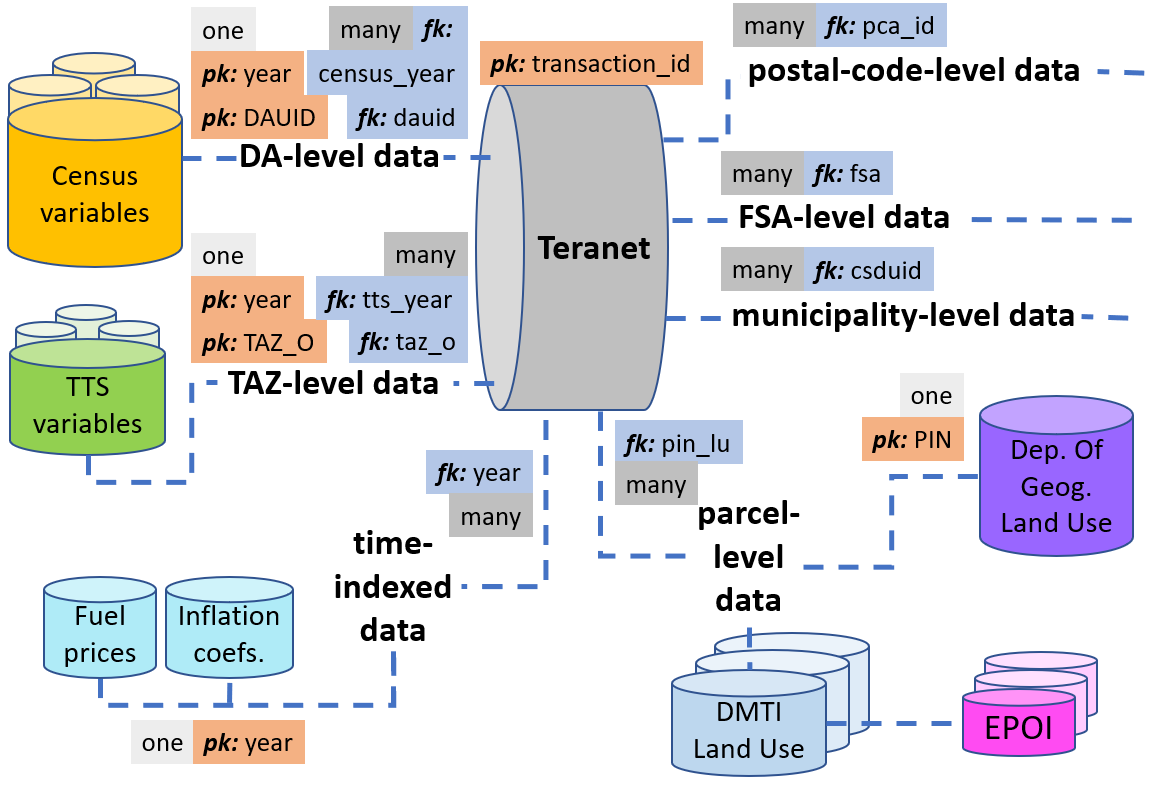
\includegraphics[width=1\linewidth,trim=0 0 0 0,clip]{data_relations.png}
    \caption{Relationships between datasets introduced during data preparation were used to set up referential integrity constraints of the new PostgreSQL database of GTHA housing market.}
    \label{fig:data_relations}
\end{figure}

Foreign keys representing temporal identifiers are generated from the registration date of each Teranet record, matching each year of Teranet records to a corresponding 5-year span covered by a Census or TTS survey, as was discussed in section~\ref{sec:termporal_relationships_between_datasets}.
Diagram of relationships between datasets via their primary and foreign keys is presented on figure~\ref{fig:data_relations}

Following the steps described above ensures that the integrity of spatial and temporal relationships is maintained when combining attributes from different data sources at Teranet transaction level.
For example, Teranet records from 2007 would be spatially joined with DMTI land use data from 2007, and are matched by their attributes 'census\_year' and 'tts\_year' to Census and TTS variables from 2006 Census and TTS surveys.
Census and TTS variables can be joined by appropriate 'dauid' and 'taz\_o' (composite foreign keys are used when joining), and thus all data sources can be spatially and temporally aligned at the level of Teranet transactions.

Relationships introduced via the operations described in this section formulate referential integrity constraints that have been used to set up a PostgreSQL database of GTHA housing market data.

\section{Dealing with outliers} \label{sec:outliers}

Outliers in both the high and the low end of the price distribution are present in Teranet's dataset:
\begin{itemize}
    \item there is a high number of transactions with very low consideration amounts (starting from a few dollars) that most likely represent transactions recording gifts of property, where some symbolic consideration amount has been set
    \item at the same time, since the dataset includes all types of property transactions, some records have very high values (in the range of millions and billions of dollars) that most likely correspond to transactions recording sales of large commercial and industrial properties or whole residential buildings
\end{itemize}

\begin{figure}[ht]
    \centering
    \begin{subfigure}{\linewidth}
        \centering
        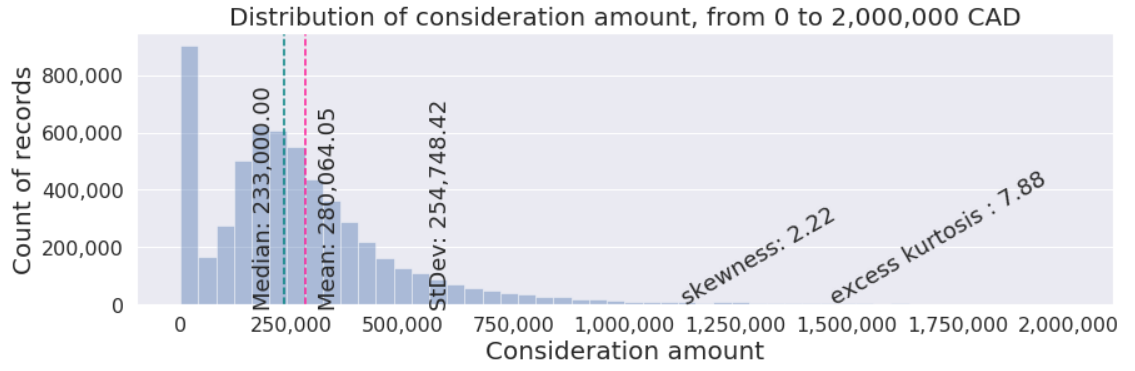
\includegraphics[width=.8\linewidth]{price_dist_raw.png}
        \caption{From 0 to 2'000'000 CAD}
    \end{subfigure}

    \begin{subfigure}{\linewidth}
        \centering
        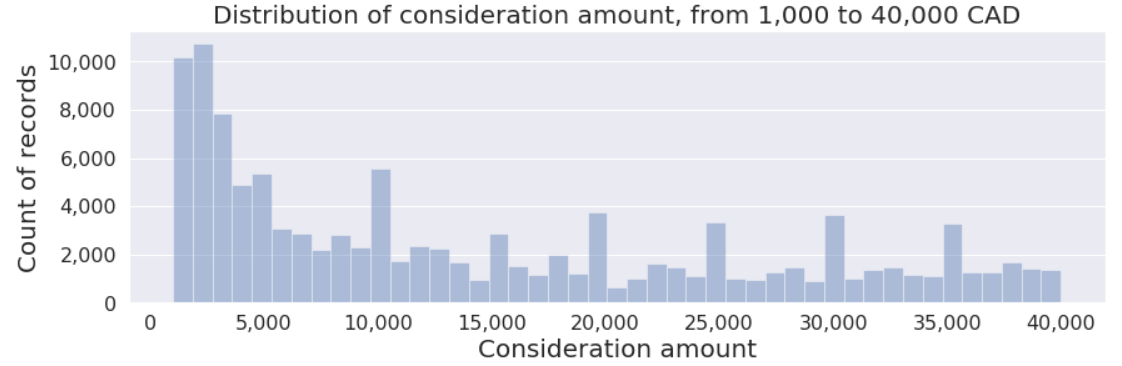
\includegraphics[width=.8\linewidth]{price_dist_zoom.png}
        \caption{From 0 to 40'000 CAD}
    \end{subfigure}
    \caption{Outliers at the bottom end of the distribution of consideration amount most likely represent gift transactions.
    Large spike can be seen on the low end of the distribution.
    Since no clear break can be identified, 10'000 CAD is proposed as the cut-off threshold to filter Teranet records.}
    \label{fig:bottom_outliers}
\end{figure}

Since low outliers represent transactions that are not useful for analysis, they are removed from the dataset.
However, there is no way to establish what constitutes a reasonable bottom cut-off threshold, as there is no criteria available and there is no distinct break in the price distribution.
Since there seems to be en exceptionally large spike of transactions with consideration amount under 10'000 CAD, they are considered to be low outliers and are removed from Teranet's dataset, further reducing the number of records from 6,803,691 to 5,188,513.

In case of the outliers on the high end of the distribution, they most likely correspond to transactions of expensive commercial and industrial property or whole residential buildings.
Since these transactions are useful for research questions concerning commercial and industrial property, they are left in the dataset and instead are marked with special features.
Since, again, there is no clear criteria for what would constitute an outlier, instead of using a single criterion, 7 different attributes are added that describe whether a record belongs to outliers according to a particular condition.

\begin{figure}[ht]
    \centering
    \begin{subfigure}{\linewidth}
        \centering
        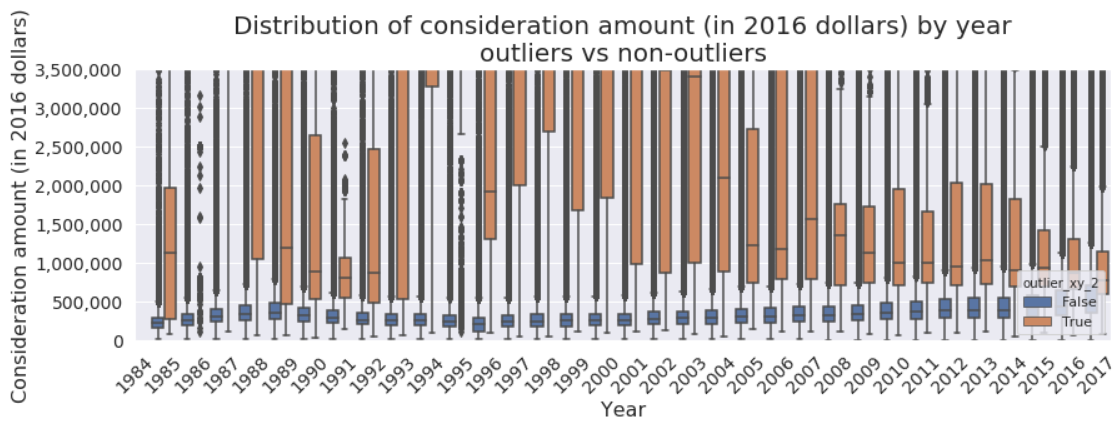
\includegraphics[width=.8\linewidth]{outliers_strict.png}
        \label{fig:top_outliers_mild}
        \caption{Outlier is 2 x median for 'xy'}
    \end{subfigure}

    \begin{subfigure}{\linewidth}
        \centering
        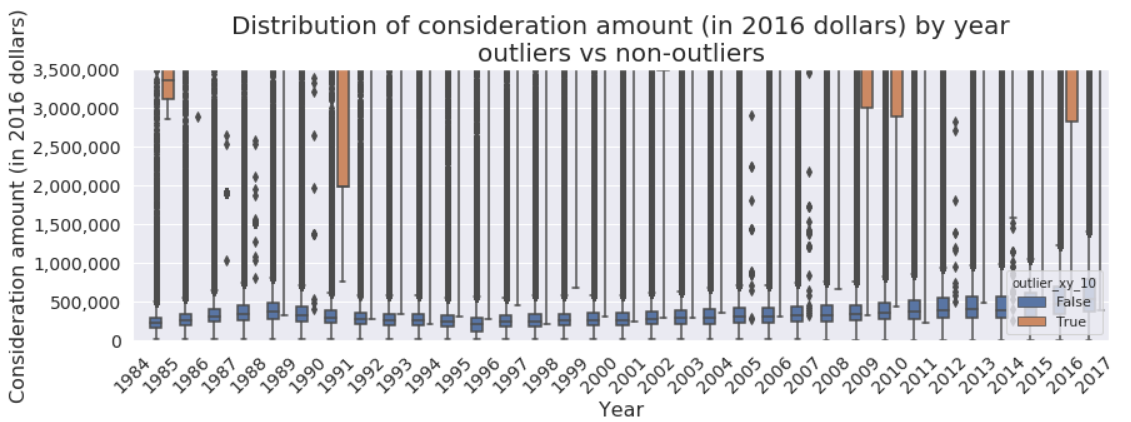
\includegraphics[width=.8\linewidth]{outliers_mild.png}
        \label{fig:top_outliers_strict}
        \caption{Outlier is 10 x median for 'xy'}
    \end{subfigure}
    \caption{Outliers at the high end of the distribution of consideration amount most likely represent commercial, industrial and transactions of whole residential buildings.
    Since these transactions can still be useful for analysis, they are kept in the dataset and instead are market with new attributes using criteria of varying strictness to define an outlier.
    The top figure presents an example where all transactions with price over 2 times greater than the median price for that 'xy' are considered to be too high, bottom figure shows an example where only records with price over 10 times greater than median for 'xy' are marked as outliers.
    7 different criteria are used in total to mark top outliers.}
    \label{fig:top_outliers}
\end{figure}

For example, feature 'outlier\_y\_10' is a Boolean variable capturing if the price of this records corrected for inflation is over 10 times the median price for the corresponding year.
New attributes identifying outliers from the high end of the distribution in layers are added to each Teranet record and are used as features by the classification algorithm.

\section{Engineering new features for classification algorithm} \label{sec:feature_engineering}

In addition to producing new keys for joining datasets, a number of new features is engineered from Teranet records to be tested with the classification algorithm (discussed in chapter~\ref{ch:ml_workflow}).
The new features are intended to give each Teranet transaction spatial and temporal "context" of the housing market dynamics by grouping Teranet records using various criteria.
For example, a feature 'xy\_prev\_sales' was added capturing the previous count of Teranet records coming from this coordinate pair;
feature 'price\_to\_med\_year' captures a ratio of consideration amount of the current record with respect to median consideration amount of all Teranet records for that year, etc.

The following features have been added to each Teranet record from 1985 to 2017 ('xy' represents 'x' and 'y' coordinates concatenated together as strings, used to group together all records from same coordinate pairs):

\begin{itemize}
    \item 'price\_2016': consideration amount corrected for inflation using the coefficients from the Inflation Calculator provided by the Bank of Canada\cite{BankofCanada2019}
    \item 'pin\_total\_sales': count of Teranet records grouped by 'pin'
    \item 'xy\_total\_sales': count of Teranet records grouped by 'xy'
    \item 'pin\_prev\_sales': rolling count of Teranet records grouped by 'pin'
    \item 'xy\_prev\_sales': rolling count of Teranet records grouped by 'xy'
    \item 'xy\_first\_sale': Boolean variable indicating whether it is the first record coming from this 'xy'
    \item 'pin\_years\_since\_last\_sale': difference in years since last record from this 'pin'
    \item 'xy\_years\_since\_last\_sale': difference in years since last record from this 'xy'
    \item 'xy\_years\_to\_next\_sale': difference in years to next record from this 'xy'
    \item 'da\_days/years\_since\_last\_sale': difference in days/years since last sale that occurred on this Dissemination Area
    \item 'xy\_sale\_next\_6m': Boolean variable indicating whether there will be another sale on this 'xy' in the upcoming 6 month
    \item 'pin\_price\_cum\_sum': cumulative sum of inflation corrected price of all Teranet records from this 'pin'
    \item 'xy\_price\_cum\_sum': cumulative sum of inflation corrected price of all Teranet records from this 'xy'
    \item 'pin\_price\_pct\_change': percentage change of price corrected for inflation from the last Teranet record from this 'pin'
    \item 'xy\_price\_pct\_change': percentage change of price corrected for inflation from the last Teranet record from this 'xy'
    \item 'price\_da\_pct\_change': percentage change of price corrected for inflation from the last Teranet record from this 'dauid'
    \item 'med\_price\_xy': median price corrected for inflation for all Teranet records from this 'xy'
%TODO finish the list of new feauters

\end{itemize}

\section{Chapter summary} \label{sec:data_preparation_summary}

All the requirements for Tidy Data and RDBMS constraints have been met by prepping the data.
%TODO write chapter summary

Characteristics of the raw Teranet dataset:
\begin{itemize}
    \item 9,039,241 rows
    \item 15 columns
\end{itemize}

Characteristics of the Teranet dataset after data preparation (described in chapter~\ref{ch:data_preparation}):
\begin{itemize}
    \item 5,188,513 rows
    \item 75 columns
\end{itemize}
